\chapter{レンズによる提案手法の検討}
\thispagestyle{empty}
\label{chap4}
\graphicspath{{chap4/figure/}}
\minitoc

\newpage
%%%%%%%%%%%%%%%%%%%%%%%%%%%%%%%%%%%%%%%%%%%%%%%%%%%%%%%%%%%%%%%%%%%%%%%%%%%%%


% ================================================== %
% section
% ================================================== %
\section{諸言}
\label{chap4_introduction}

本章では5章のミラー測定実験に先立って、ほぼ理想的と言える集光光学系に対して3章で提案された手法による計測実験を行い、その正当性を検証する。
具体的な方法としては、平行光に対して輪帯状の開口を入れ、さらにレンズによって集光することで、輪帯状の集光球面波を作ることができ、擬似的にミラー下流端面を再現する。
再現された擬似的な輪帯に対して位相回復法が適用出来れば、細い輪帯形状の波面回復法に対して提案手法が有効的であることがいえ、また本研究の測定対象である天文用Wolterミラーに対してもその適用可能性が大きいということが言える。
また、1層のWolterミラーの波面計測のための手法検討に加えて、Nested Wolterミラーにも同手法が適用可能であるかどうかを検討するための実験を行う。
現時点では入手性の観点から実際のNested Wolterミラーを計測することは難しいが、Nested Wolterミラーの集光波面を模倣した輪帯に対して位相回復法が機能すれば、十分に応用可能であることの根拠を与える。
\ref{chap4_experiment_setup}節では、実験の構成およびそれに含まれる各光学素子のパラメータ等について示す。


\clearpage
% ================================================== %
% section
% ================================================== %
\newpage

\section{実験の構成および設計パラメータ}
\label{chap4_experiment_setup}

\ref{chap4_introduction}節で述べたとおり、本章ではほぼ理想的な輪帯上の集光波面を擬似的に生成し、これに対して波面計測を行う。
輪帯上の集光波面は、図\ref{fig:psuedo_focusing_ring_model}に示すように輪帯アパーチャ及び集光レンズによって生成される。

\begin{figure}[!ht]
\centering
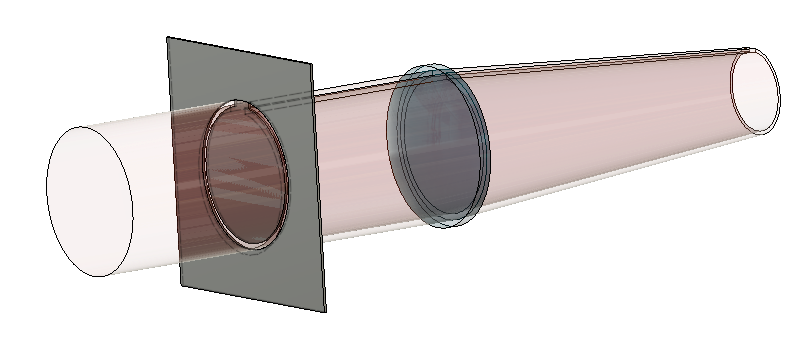
\includegraphics[width=13cm]{psuedo_focusing_ring.png}
\caption{疑似的な輪帯状集光ビームの生成}
\label{fig:psuedo_focusing_ring_model}
\end{figure}

疑似輪帯を用いた計測実験は、本来の測定対象であるWolterミラーと同様の光学的パラメータで構成されるべきだが、入手性の問題からここではレンズとして口径は異なるがNAがWolterミラーのそれとほぼ等しいレンズを用いる。
用いたレンズのパラメータは表\ref{tb:focusing_lens_params}に示す通りである。

\begin{table}[h]
\begin{center}
  \begin{tabular}{|c|c|} \hline
    パラメータ & 値 \\ \hline
    直径 & 30.0 mm  \\
    焦点距離 & 1000.000 mm \\
    設計波長 & 541.6 nm \\ \hline
  \end{tabular}
  \caption{レンズの設計パラメータ}
  \label{tb:focusing_lens_params}
\end{center}
\end{table}

これに合わせて、輪帯開口および位相回復に用いるピンホールを図\ref{fig:lens_pinhole_ring_aperture}の用に設計した。

\begin{figure}[!ht]
\centering

\subfloat[輪帯アパーチャ]{
    \centering
    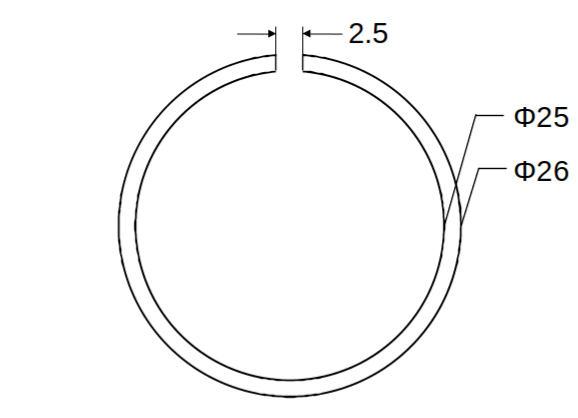
\includegraphics[width=6cm]{ring_aperture.png}
    \label{fig:lens_ring_aperture}
}
\subfloat[ピンホール]{
    \centering
    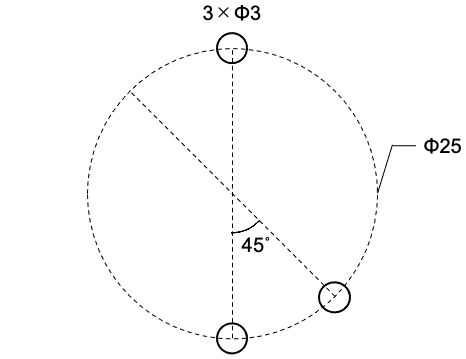
\includegraphics[width=6cm]{pinhole_arrangement.png}
    \label{fig:lens_pinhole_arrangement}
}
\caption[]{設計図面}
\label{fig:lens_pinhole_ring_aperture}
\end{figure}

\clearpage
% ================================================== %
% section
% ================================================== %
\newpage


\section{疎条件を利用した位相回復の結果}
回復計算に用いたパラメータは以下の通りである。

回復計算が収束しなかった。


\clearpage
% ================================================== %
% section
% ================================================== %
\newpage

\section{下流端走査によるタイコグラフィの結果}


\subsection{半周のみ走査した場合のタイコグラフィの結果}

\subsection{繰り返し計測の結果}

像が回復できることが確認されたため、さらに10回の繰り返し計測を行い、繰り返し再現性およびその波面計測の精度を確認する。


\clearpage
% ================================================== %
% section
% ================================================== %
\newpage

\section{Nested Wolterミラーに対する下流端走査型位相回復法の検証}

1層の場合と同様に、輪帯状の集光波面が同心円状に2つ存在するような状況を擬似的に作り出し、これを計測する。
アパーチャとピンホールの設計を図\ref{fig:lens_nested_pinhole_ring_aperture}に示す。

\begin{figure}[!ht]
\centering

\subfloat[輪帯アパーチャ]{
    \centering
    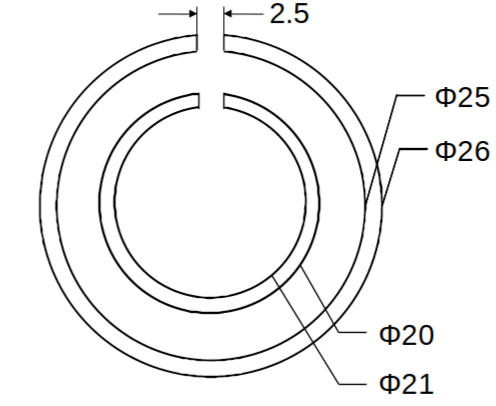
\includegraphics[width=6cm]{nested_ring_aperture.png}
    \label{fig:lens_nested_ring_aperture}
}
\subfloat[ピンホール]{
    \centering
    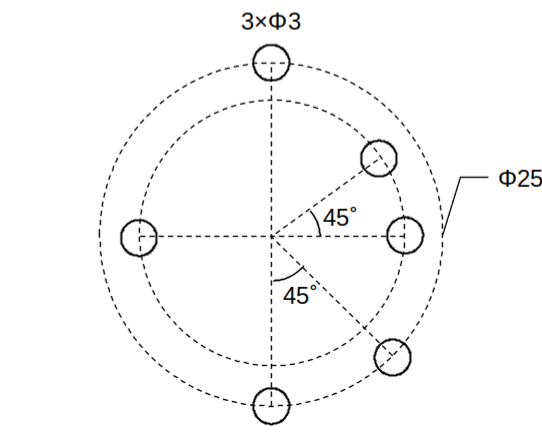
\includegraphics[width=6cm]{nested_pinhole_arrangement.png}
    \label{fig:lens_nested_pinhole_arrangement}
}
\caption[]{疑似Nested Wolter計測用の設計図面}
\label{fig:lens_nested_pinhole_ring_aperture}
\end{figure}

\subsection{結果}

回復された波面の強度分布を図\ref{fig:result_nested_restored_abs}に示す。

\begin{figure}[!ht]
\centering
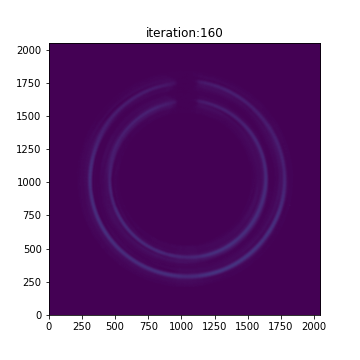
\includegraphics[width=6cm]{result_nested/restored_abs.png}
\caption{疑似的な輪帯状集光ビームの生成}
\label{fig:result_nested_restroed_abs}
\end{figure}



\clearpage
% ================================================== %
% section
% ================================================== %
\newpage


\section{結論}
\label{chap4_conclusion}


%%%%%%%%%%%%%%%%%%%%%%%%%%%%%%%%%%%%%%%%%%%%%%%%%%%%%%%%%%%%%%%%%%%%%%%%%%%%%
%%% Local Variables:
%%% mode: katex
%%% TeX-master: "../thesis"
%%% End:
